\documentclass[english]{article}
\usepackage[T1]{fontenc}
\usepackage[latin9]{inputenc}
\usepackage{babel}
\usepackage{graphicx}
\graphicspath{{images/}}
\begin{document}

\section{Specific Requirement}

\subsection{External interfaces}

\subsection{UseCase Diagram}

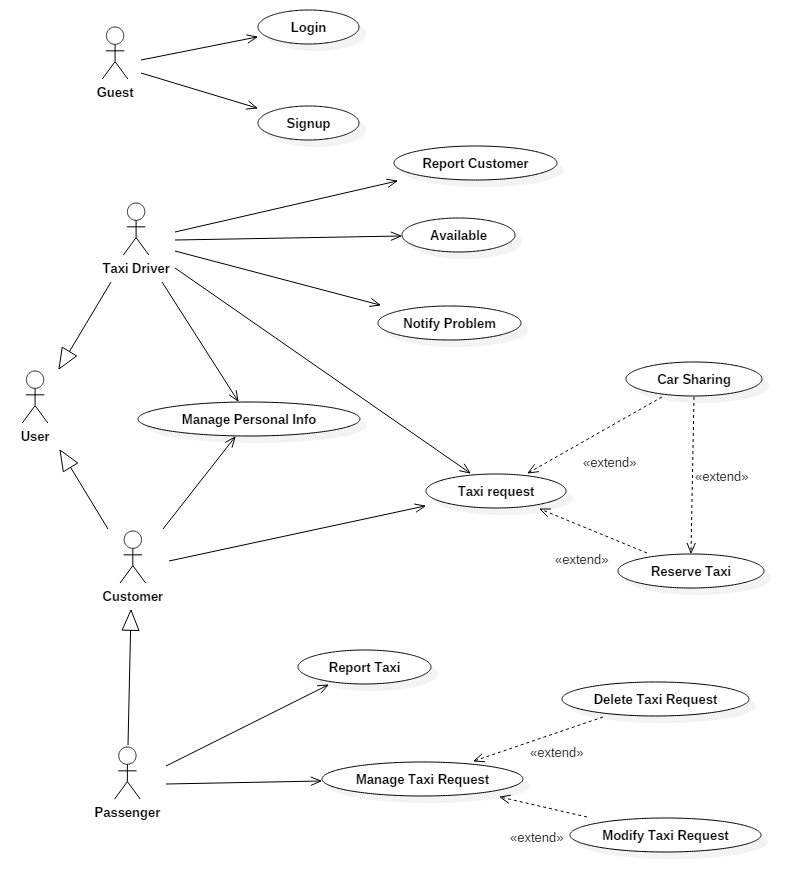
\includegraphics[width=\textwidth]{UseCase}

\subsection{Scenario}

\emph{Adam need to take a taxi}

\subsubsection{Signup}
Adam is new into the System and wants to signup. He requires the Passenger registration page, fills the form and submit the request to the System. If the email and username are unique the System confirms to Adam the successful of the operations and redirect Adam to the Login page, otherwise it display an error message

\subsubsection{Login}
Adam, now registered, insert the username and password in the login form and click the login button, the System checks the informations and, in case of correct informations, redirect Adam to his own User profile page, otherwise shows an error message

\emph{Hector is a Taxi Driver logged into the System}

\subsubsection{Available}
Hector, logged into the System, start his working day opening his Taxi Driver profile page and telling his availability to the System. The System change the queue and notify the position (2nd) in the queue to Hector.

\subsubsection{Taxi Request}
Adam, now logged into the System, book a Taxi for the 5PM (now 3PM) inserting informations in the Taxi Request page (previously required from the system) and submit the data into the System. Now the System check the informations, if are wrongs display to Adam a message with the error, otherwise start asking to the Taxis queue. The System ask the request to the first of the queue, who reject the request and is moved at the end of the queue. The System repeat the operation with the new first of the queue, Hector now confirm the request and take in charge the request. The System now confirm the successful to Adam, and is now a Passenger.

\subsubsection{Manage Taxi Request}
Adam opens the Manage Taxi Request page to change the book hour to 6PM, change the hour and, because are missing at most two hours, the System change the information and notify the change to Hector.

\subsubsection{Report Taxi}
Hector takes Adam, during the ride Hector lights a cigarette and Adam open the Report Taxi page to complain this behavior, fill the form with the informations and submit this into the System. The System updates the Taxi Driver informations and confirm the end of the operation to Adam.

\subsubsection{Report User}
After the ride, Adam annoyed for the behavior of Hector refused to pay the Taxi Driver. Hector open the report User page, fills the informations and submit the data. The System updates the User informations adding a negative report and notify the end of the operation to Hector. 

\subsubsection{Manage Personal Informations}
Adam opens his User Profile page, click on the edit button and change his email, submit the new informations. The System checks the informations, if are right update the Adam profile and notify the success of the operation to Adam.

\emph{Samuel is a Taxi Driver logged into the System, available in the zone which Hector is now}

\subsubsection{Report Problem}
Hector during a ride, has a problem with his taxi motor and thought the Report Problem page report the problem filling the form and submitting. The System insert the problem and ask to Hector if needs a new Taxi. Hector positively answer to the request and the System ask to the first of the queue to reach Hector and his Passenger. Samuel, the first of the queue, accept the request and reach his colleague.

\subsection{Functions}

\subsubsection{Signup}

\begin{tabular}{lp{8cm}}
\hline
Actors & Guest \\
\hline
Preconditions &  The Guest is not registered into the system \\
\hline
Execution Flow &  
		\begin{enumerate}
			\item The Guest request the registration page
			\item The System requires the Signup information
			\item The Guest fill the form and submit the request
			\item The System check the uniqueness of the Username and E-Mail
			\item The System create the User (or Taxi drive) profile
			\item The System send the confirm the the Guest
		\end{enumerate} 
	\\ 
\hline
Postconditions & The guest is now a User o a Taxi driver \\
\hline
Exceptions & The E-Maill or username are not unique or, in the case of taxi driver signup, the licenses are not valid
\end{tabular}

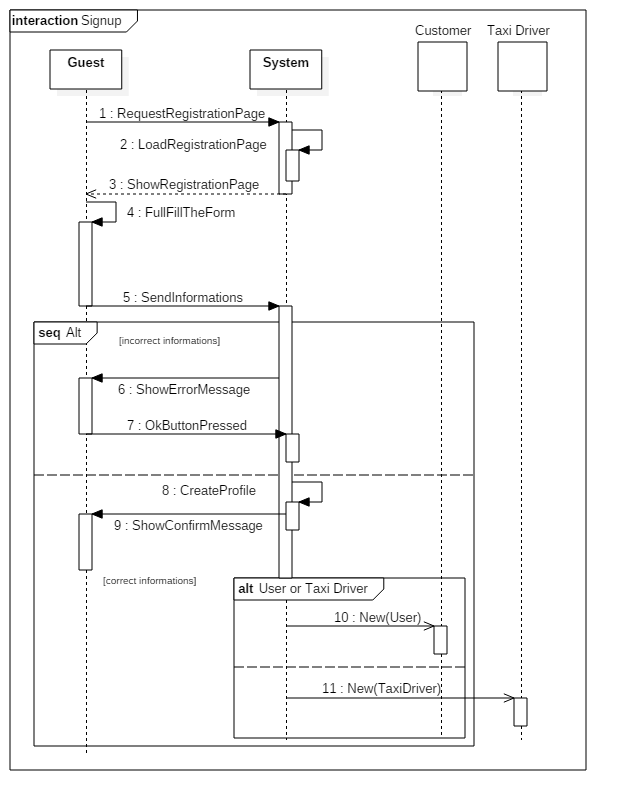
\includegraphics[width=\textwidth]{Signup}

\subsubsection{Login}

\begin{tabular}{lp{8cm}}
\hline
Actors & Guest \\
\hline
Preconditions &   The Guest has already a profile into the System\\
\hline
Execution Flow &  
		\begin{enumerate}
			\item The Guest request the login page
			\item The System requires the Login information (Username, Password)
			\item The Guest fill the form and submit the request
			\item The System check the Username and Password
			\item The System send the confirmation of Login
			\item The Guest is logged into the System
			\item The Guest is redirected to the User profile Page
		\end{enumerate} 
	\\ 
\hline
Postconditions & The guest is now a User or Taxi Driver \\
\hline
Exceptions & The Usename, password couple is incorrect, so the Guest cannot log in
\end{tabular}

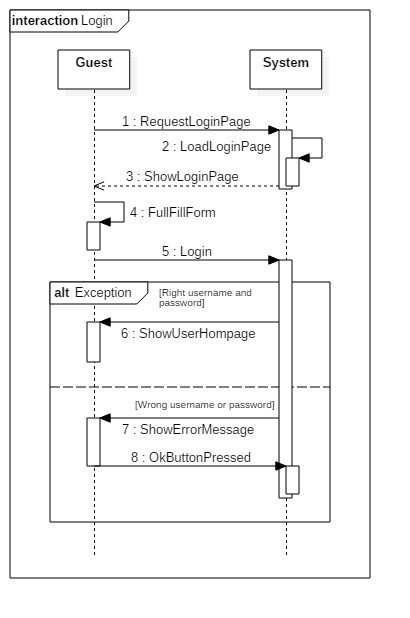
\includegraphics[width=\textwidth]{Login}

\subsubsection{Available}

\begin{tabular}{lp{8cm}}
\hline
Actors & Taxi Driver \\
\hline
Preconditions & \\
\hline
Execution Flow &  
		\begin{enumerate}
			\item The Taxi Driver request the Taxi profile page
			\item The System returns the personal informations of the Taxi
			\item The Taxi Driver notify the availability to the System
			\item The System update the local queue
			\item The System confirm the request to the Taxi Driver
		\end{enumerate} 
	\\ 
\hline
Postconditions & The Taxi Driver is now Available \\
\hline
Exceptions & 
	\begin{itemize} 
		\item The Taxi Driver is located in a invalid zone
		\item The Taxi Driver is carrying a Passenger
		\item The Taxi Driver is yet available
	\end{itemize}
\end{tabular}

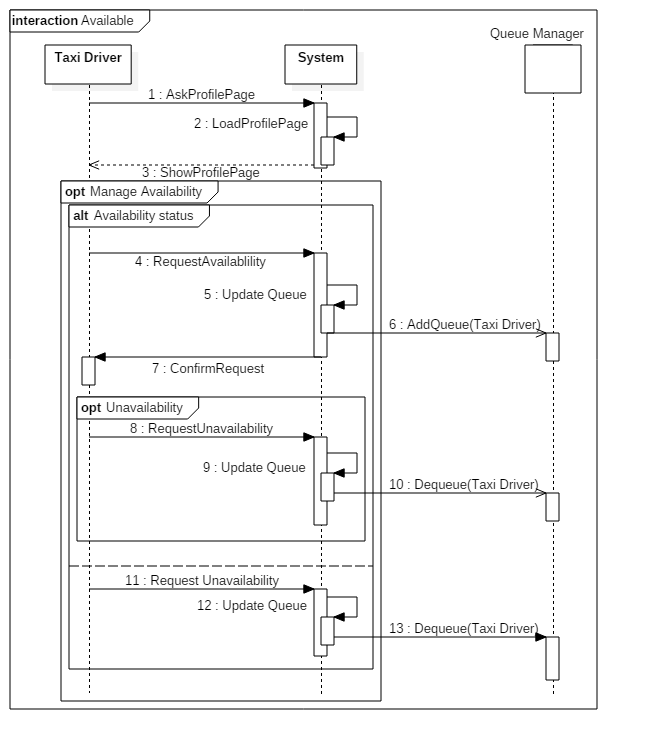
\includegraphics[width=\textwidth]{Available}

\subsubsection{Taxi Request}

\begin{tabular}{lp{8cm}}
\hline
Actors & User, Taxi Driver \\
\hline
Preconditions & The User should not be banned \\
\hline
Execution Flow &  
		\begin{enumerate}
			\item The Guest request the Taxi Request page
			\item The System requires the type of request the User wants to perform
			\item The User provide the choice to the System
			\item The System ask for the information to perform the choose request
			\item The User fill the form and send the information to the System
			\item The System forward the request to the first Taxi Driver of the local queue
			\item If the Taxi Driver answer positively to the request he take in charge the User, otherwise he deny the request
			\item If the Taxi Driver answered positively the System notify to the User the incoming taxi and change the availability of the Taxi Driver, otherwise the System update the queue and forward the request to the new first of queue until the queue is not repeated
			\item If there are no Taxis available the System notify to the User the unavailability
		\end{enumerate} 
	\\ 
\hline
Postconditions & If the request has positively response the User is now a Passenger \\
\hline
Exceptions & 
	\begin{itemize} 
		\item The User provides incorrect informations in the request form
		\item The User is not into a valid position (\emph{e.g. outside the city})
	\end{itemize}
\end{tabular}

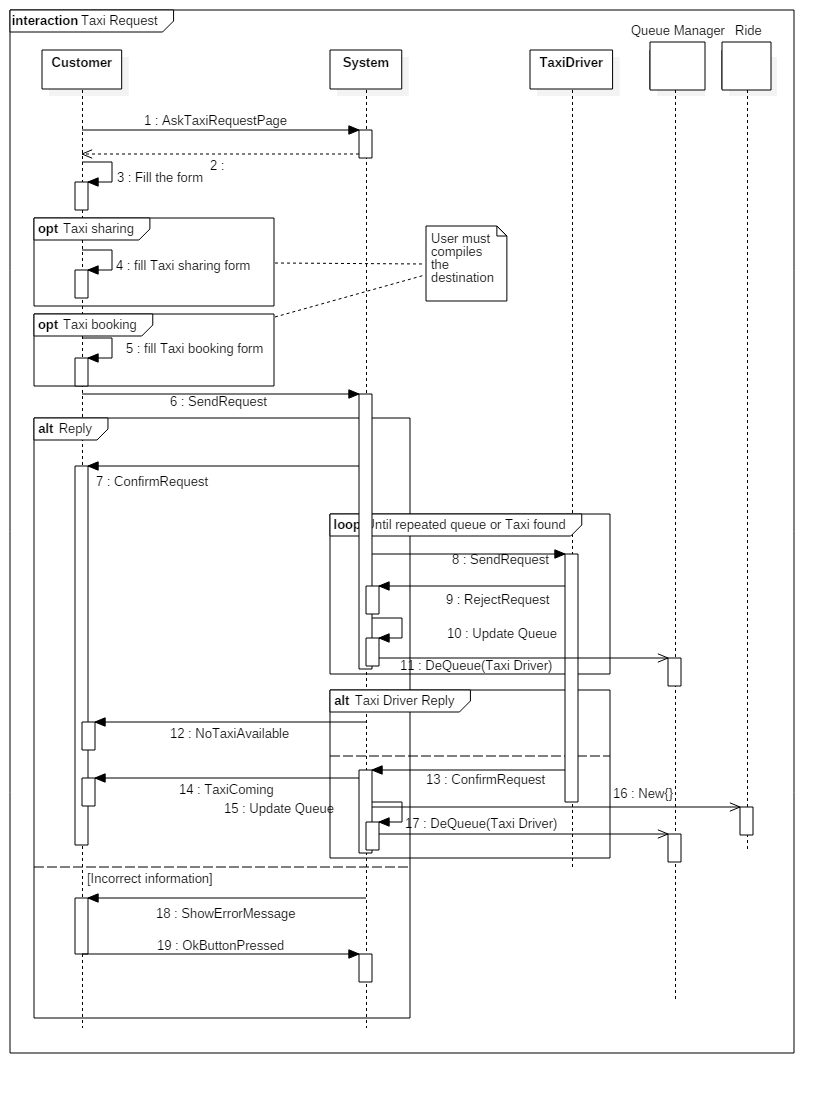
\includegraphics[width=\textwidth]{TaxiRequest}

\subsubsection{Manage Taxi Request}

\begin{tabular}{lp{8cm}}
\hline
Actors & Passenger \\
\hline
Preconditions &  \\
\hline
Execution Flow &  
		\begin{enumerate}
			\item The Passenger request the Taxi Request Management page
			\item The System load the page and return it to the Passenger
			\item The Passenger can modify the Request full filling the modify Request
			\item The System modify the request and return a confirm to the Passenger
			\item The Passenger can delete the request, submitting the operation to the System
			\item The System update the queue and return a confirmation to the Passenger
		\end{enumerate} 
	\\ 
\hline
Postconditions & 
	\begin{itemize}
		\item If the Passenger choose to modify the Request, the request is updated 
		\item If the Passenger choose to delete the Request, the request is canceled and the taxi is now in queue
	\end{itemize} \\
\hline
Exceptions & 
	\begin{itemize} 
		\item The Passenger provides incorrect informations in the modify request form
		\item The Passenger cancel the request too late
	\end{itemize}
\end{tabular}

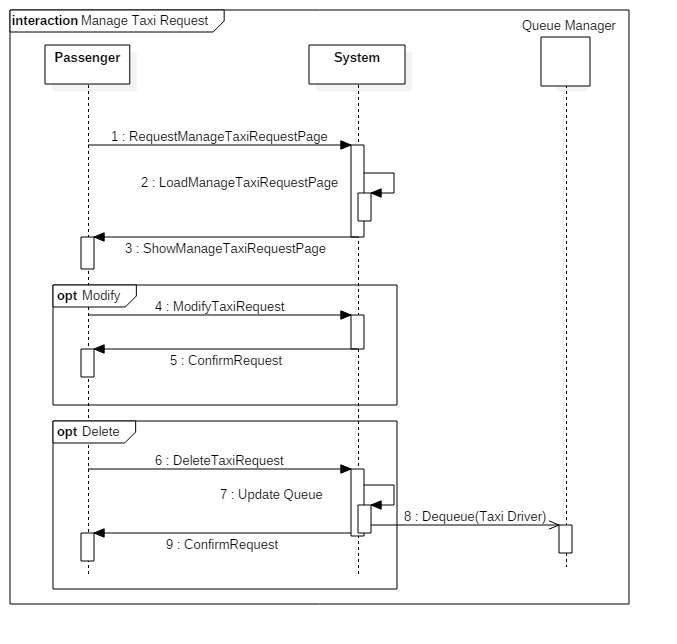
\includegraphics[width=\textwidth]{ManageTaxiRequest}

\subsubsection{Report Taxi}

\begin{tabular}{lp{8cm}}
\hline
Actors & Passenger \\
\hline
Preconditions & \\
\hline
Execution Flow &  
		\begin{enumerate}
			\item The Passenger request the Report Taxi page
			\item The System elaborate the request and ask to the Passenger the report information
			\item The Passenger fill the form and submit the report
			\item The System check the data obtained
			\item The System update the Taxi Driver informations
			\item The System notify to the Passenger the successful of the operation
		\end{enumerate} 
	\\ 
\hline
Postconditions & The Taxi Driver is reported by the current Passenger \\
\hline
Exceptions & The Passenger provides wrong informations in the report form
\end{tabular}

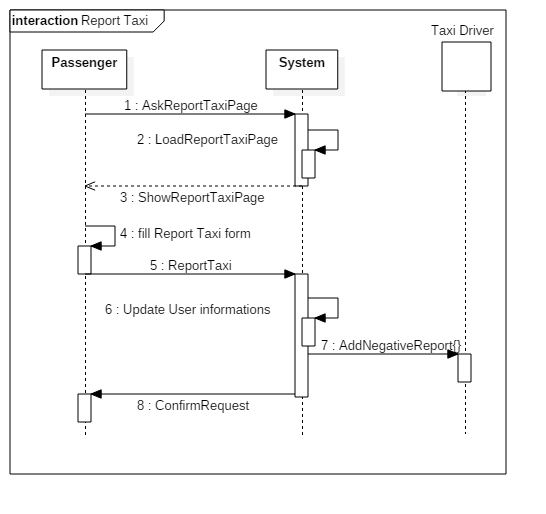
\includegraphics[width=\textwidth]{ReportTaxi}

\subsubsection{Report User}

\begin{tabular}{lp{8cm}}
\hline
Actors & Taxi Driver \\
\hline
Preconditions & The Taxi Driver should had carried the User past 24 hours \\
\hline
Execution Flow &  
		\begin{enumerate}
			\item The Taxi Driver request the Report User page
			\item The System elaborate the request and ask to the Taxi Driver the report information
			\item The Taxi Driver fill the form and submit the report
			\item The System check the data obtained
			\item The System update the User informations
			\item The System notify to the Taxi Driver the successful of the operation
		\end{enumerate} 
	\\ 
\hline
Postconditions & The User is reported by the Taxi Driver \\
\hline
Exceptions & The Taxi Driver provides wrong informations in the report form
\end{tabular}

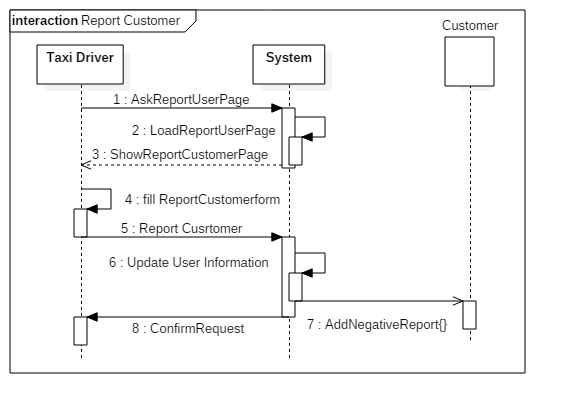
\includegraphics[width=\textwidth]{ReportUser}

\subsubsection{Manage Personal Informations}

\begin{tabular}{lp{8cm}}
\hline
Actors & User or Taxi Driver \\
\hline
Preconditions & \\
\hline
Execution Flow &  
		\begin{enumerate}
			\item The User (or Taxi Driver) request the User profile page
			\item The System returns the personal informations of the User (or Taxi Driver)
			\item The User (or Taxi Driver) can request the edit of the profile
			\item The System return the editable informations of the profile
			\item The User (or Taxi Driver) can edit those data and send the changes to the System
			\item The System check the correctness of the new Informations
			\item If the informations are correct send the Change Confirm to the User (or Taxi Driver), otherwise send back an error message
		\end{enumerate} 
	\\ 
\hline
Postconditions & If the User request a modify profile and submit correct informations the Profile is changed \\
\hline
Exceptions & The User provides wrong informations
\end{tabular}

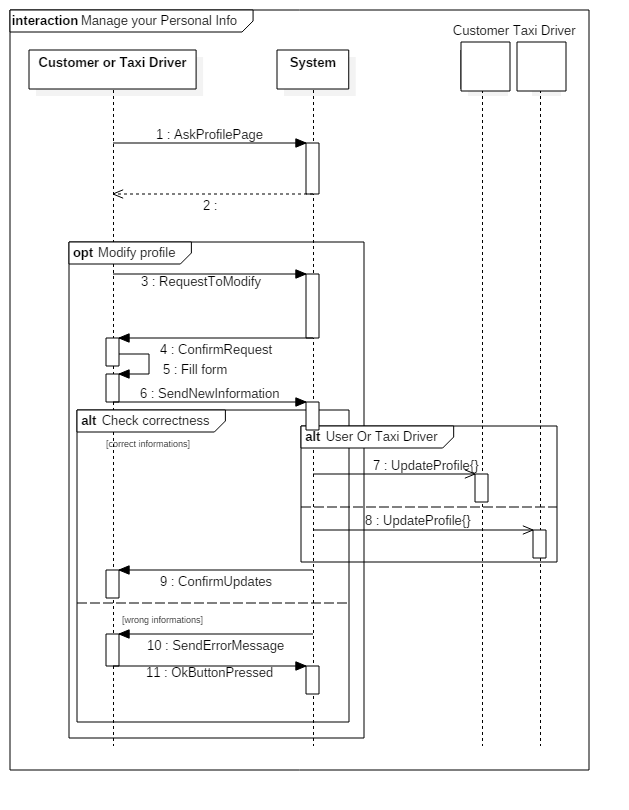
\includegraphics[width=\textwidth]{ManageInformation}

\subsubsection{Notify Problem}

\begin{tabular}{lp{8cm}}
\hline
Actors & Taxi Driver \\
\hline
Preconditions & \\
\hline
Execution Flow &  
		\begin{enumerate}
			\item The Taxi Driver request the Report Problem page
			\item The System returns the page of the Report requiring problem informations
			\item The Taxi Driver fill the form and send the information
			\item The Taxi Driver can request another Taxi for the User who is carrying (if is carrying one)
			\item If the Taxi Driver request another Taxi the System looks for a available Taxi Driver
			\item If exist an available Taxi change the carrier of the User with the new Taxi Driver and send him, otherwise notify the unavailability
			\item The System return the success of the operation
		\end{enumerate} 
	\\ 
\hline
Postconditions & The problem is submitted into the System \\
\hline
Exceptions & 
	\begin{itemize}
		\item The Taxi Driver is located in a invalid zone
		\item The Taxi Driver fill the form with wrong informations
	\end{itemize}
\end{tabular}

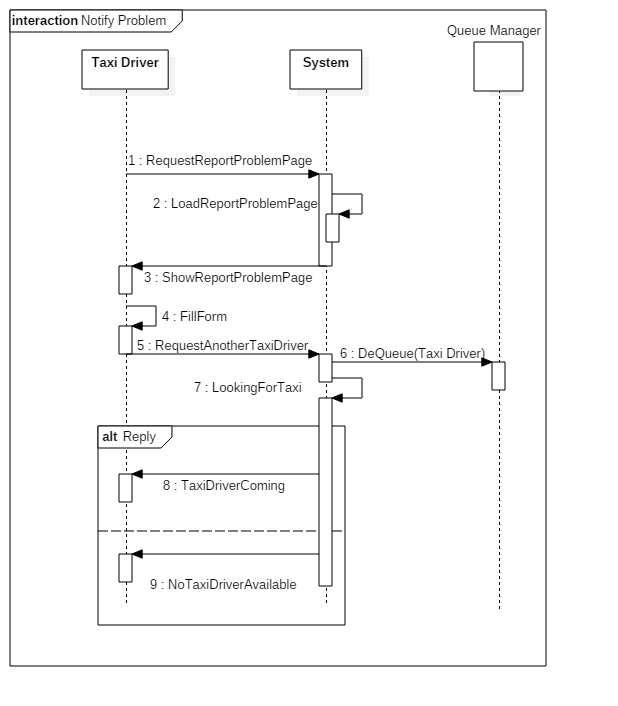
\includegraphics[width=\textwidth]{NotifyProblem}

\subsection{Performance requirements}
	\begin{itemize}
		\item The System should support at least all the Taxi Driver registered into the City Database
		\item The System should elaborate User incoming informations
		\item The System should provide the faster path for each ride
		\item The System should calculate the final price of the ride with a maximum error of 10\%
		\item The System should provide to a Passenger the arrival time (maximum error 20\%) and change the path in case of traffic
	\end{itemize}
	
\subsection{Logical database requirements}

\subsection{Design constraints}
	\begin{itemize}
		\item GPS precision limitations: average 3m error
		\item Internet congestion
	\end{itemize}

\subsection{Standards compliance}

\subsection{Software system attributes}

\subsection{Reliability}

\subsection{Availability}

\subsection{Security}
	\begin{itemize}
		\item SSL connection over the web
		\item Username and password to identify the User and Taxi Driver
		\item All the Operation are logged into the System
		\item The data stored inside the secondary store are encrypted
		\item The System databases has consistency check, data integrity check
	\end{itemize}

\subsection{Maintainability}

\subsection{Portability}

\subsection{Organizing the specific requirements}

\subsection{System mode}

\subsection{User class}
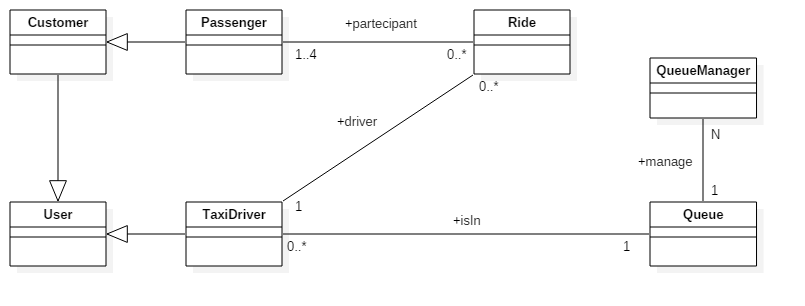
\includegraphics[width=\textwidth]{ClassDiagram}

\subsection{Objects}

\subsection{Feature}

\subsection{Stimulus}

\subsection{Response}

\subsection{Functional hierarchy}

\subsection{Additional comments}

\end{document}